\documentclass[../notes.tex]{subfiles}

\pagestyle{main}
\renewcommand{\chaptermark}[1]{\markboth{\chaptername\ \thechapter\ (#1)}{}}
\setcounter{chapter}{7}

\begin{document}




\chapter{Symmetric Group Representation Formulations}
\section{Specht Modules are Irreducible and Well-Defined}
\begin{itemize}
    \item \marginnote{11/13:}Announcements.
    \begin{itemize}
        \item This week's homework is the next to last one.
    \end{itemize}
    \item Review.
    \begin{itemize}
        \item Miracuously, we can understand all representations of $S_n$.
        \item We start with partitions $\lambda$ that are defined a certain way. We visualize them with Young diagrams.
        \item The number of partitions of $n$ is equal to the number of conjugacy classes in $S_n$ is equal to the number of irreps in $S_n$.
        \begin{itemize}
            \item It is a special feature of $S_n$ that this is true.
        \end{itemize}
        \item How do we construct the irreducible representation $V_\lambda$ due to $\lambda$?
        \begin{itemize}
            \item Consider $(4,2,1)'=(3,2,1,1)$ as an example (recall the definition of an inverse partition).
            \item Take Vandermonde determinants (recall the explicit definition of these, too) of column elements and multiply them together.
            \item Then we define $V_\lambda$\footnote{Something about $V_\lambda=\C[S_n]$?? I though we were "just say NO!"-ing this usual construction, though?} to be the subspace of the polynomial space $\C[x_1,\dots,x_n]$ that is spanned by the Vandermonde determinants polynomial and all actions of $S_n$ on it.
            \item In particular, take Vandermonde determinant of variables corresponding to the successive columns to obtain
            \begin{equation*}
                \Delta(x_1,\dots,x_{\lambda_1'})\Delta(x_{\lambda_1'+1},\dots,x_{\lambda_2'})\cdots\Delta(x_{\lambda_{k-1}'+1},\dots,\lambda_k')
            \end{equation*}
            \item Thus, in our specific example, we let $\C[S_n]$ act on $(x_1-x_2)(x_1-x_3)(x_2-x_3)(x_4-x_5)$.
        \end{itemize}
    \end{itemize}
    \item One more example.
    \begin{itemize}
        \item $\lambda=(2,2)$.
        \item Let $\C[S_4]$ act on $(x_1-x_2)(x_3-x_4)$.
        \item Then
        \begin{equation*}
            V_\lambda = \inp{(x_1-x_2)(x_3-x_4),(x_1-x_3)(x_2-x_4),(x_1-x_4)(x_2-x_3)}
        \end{equation*}
        \item But we're expecting a 2D representation. Indeed, we get one because if we define the first term above to be $a$ and the second to be $b$, then the third is $b-a$:
        \begin{align*}
            b-a &= [(x_1-x_3)(x_2-x_4)]-[(x_1-x_2)(x_3-x_4)]\\
            &= [x_1x_2-x_1x_4-x_2x_3+x_3x_4]-[x_1x_3-x_1x_4-x_2x_3+x_2x_4]\\
            &= x_1x_2+x_3x_4-x_1x_3-x_2x_4\\
            &= (x_1-x_4)(x_2-x_3)
        \end{align*}
        \item Consequence of the above: There are only two linearly independent polynomials herein.
        \item Thus, the final Specht module is
        \begin{equation*}
            V_\lambda = \langle\underbrace{(x_1-x_2)(x_3-x_4)}_a,\underbrace{(x_1-x_3)(x_2-x_4)}_b\rangle
        \end{equation*}
        \item Now we calculate entries in the character table as follows: See how representatives of conjugacy classes like $(12)$ and $(123)$ acts on $a,b$ via matrices, and then calculate traces of these matrices.
        \begin{itemize}
            \item For example, using the definitions of $a,b$ from above, we can see that
            \begin{align*}
                (12)\cdot a &= (12)\cdot(x_1-x_2)(x_3-x_4)
                    = (x_2-x_1)(x_3-x_4)
                    = -(x_1-x_2)(x_3-x_4)
                    = -a\\
                (12)\cdot b &= (12)\cdot(x_1-x_3)(x_2-x_4)
                    = (x_2-x_3)(x_1-x_4)
                    = (x_1-x_4)(x_2-x_3)
                    = b-a
            \end{align*}
            \item In matrix form, the above equations become
            \begin{equation*}
                \begin{bmatrix}
                    -a\\
                    b-a\\
                \end{bmatrix}
                = \underbrace{
                    \begin{bmatrix}
                        -1 & 0\\
                        -1 & 1\\
                    \end{bmatrix}
                }_{\rho(12)}
                \begin{bmatrix}
                    a\\
                    b\\
                \end{bmatrix}
            \end{equation*}
            \item Thus, $\chi(12)=\tr[\rho(12)]=0$.
            \item Similarly, we can calculate that
            \begin{equation*}
                \begin{bmatrix}
                    b-a\\
                    -a\\
                \end{bmatrix}
                = \underbrace{
                    \begin{bmatrix}
                        -1 & 1\\
                        -1 & 0\\
                    \end{bmatrix}
                }_{\rho(123)}
                \begin{bmatrix}
                    a\\
                    b\\
                \end{bmatrix}
            \end{equation*}
            so $\chi(123)=-1$.
        \end{itemize}
        \item One of the HW problems is to do exactly this for $S_4$ just for practice.
    \end{itemize}
    \item Today: A theorem that proves the $V_\lambda$ are irreducible (as our notation would suggest), and a theorem that proves the $V_\lambda$ are well-defined (i.e., only one $V_\lambda$ can be constructed from each $\lambda$).
    \item Note: $V_\lambda$ is a \textbf{Specht module} and the original polynomial constructed is the \textbf{Specht polynomial}.
    \item We now build up to the theorems.
    \item \textbf{Degree} (of a Specht polynomial): The degree of the given polynomial as defined in Lecture 7.1. \emph{Denoted by} $\bm{d(\lambda)}$. \emph{Given by}
    \begin{equation*}
        d(\lambda) = \sum_{i=1}^{k'}\frac{\lambda_i'(\lambda_i'-1)}{2}
    \end{equation*}
    \item Let $R_d$ denote the subset of $\C[x_1,\dots,x_n]$ consisting of polynomials of degree $d$.
    \begin{itemize}
        \item Recall also that as a definition, $R_d=S^d(V_\text{perm}^*)$.
        \item Note that if $d=d(\lambda)$, then $V_\lambda\subset R_d$.
    \end{itemize}
    \item Lemma: Let $\lambda$ be a partition of $n$, $d=d(\lambda)$, $R_d$ be the subset of $\C[x_1,\dots,x_n]$ consisting of polynomials of degree $d$, and $V_\lambda$ be the Specht module of $\lambda$. Then
    \begin{equation*}
        \Hom_{S_n}(V_\lambda,R_d) \cong \C
    \end{equation*}
    \begin{proof}
        Let $f\in\Hom_{S_n}(V_\lambda,R_d)$ be arbitrary, let $\Delta(x_1,\dots,x_{\lambda_1'})\Delta(x_{\lambda_1'+1},\dots,x_{\lambda_2'})\dots$ be an arbitrary element of $V_\lambda$, and let
        \begin{equation*}
            P(x_1,\dots,x_n) := f(\Delta(x_1,\dots,x_{\lambda_1'})\Delta(x_{\lambda_1'+1},\dots,x_{\lambda_2'})\dots)
        \end{equation*}
        By definition, the degree of $P$ is $d$. Additionally, because $f$ is a morphism of $S_n$-representations as an element of $\Hom_{S_n}(V_\lambda,R_d)$, we have that $f$ is linear and hence, since the argument of $f$ is antisymmetric in $x_1,\dots,x_{\lambda_1'}$, so $P$ similarly antisymmetric. $P$ is also antisymmetric in $x_{\lambda_1'+1},\dots,x_{\lambda_2'}$. In fact, $P$ is antisymmetric in all such sets all the way up to $x_{\lambda_{k'-1}'+1},\dots,x_{\lambda_{k'}'}$. It follows that $P(x_1,\dots,x_n)$ is divisible by $\Delta(x_1,\dots,x_{\lambda_i'})$, etc., i.e., all Vandermonde determinants. Thus, $P(x_1,\dots,x_n)$ is divisible by the product, which is the $d$-degree Specht polynomial argument of $f$. It follows that
        \begin{equation*}
            P(x_1,\dots,x_n) = u\cdot\Delta(x_1,\dots,x_{\lambda_1'})\Delta(x_{\lambda_1'+1},\dots,x_{\lambda_2'})\dots
        \end{equation*}
        from which it follows that $f=uI$. This implies the claim via the isomorphism $f\mapsto u$.
    \end{proof}
    \item Theorem 1: $V_\lambda$ is irreducible.
    \begin{proof}
        Let $V_\lambda=\bigoplus W_i^{n_i}$ and $R_d=\bigoplus W_i^{m_i}$, where the $W_i$ are all irreps. From previous classes, we have a nice way to compute a morphism of $S_n$-representations $V_\lambda\to R_d$: Explicitly, we apply Schur's lemma to find that the only acceptable constituent morphisms are those which send $W_i\to W_i$. Thus, $\dim\Hom_{S_n}(V_\lambda,R_d)=\sum n_im_i$. (Any transformation from $W_i^{n_i}$ to $W_i^{m_i}$ has the form of a $m_i\times n_i$-blocked matrix, so there are $n_im_i$ degrees of freedom.) But by the lemma, $\dim\Hom_{S_n}(V_\lambda,R_d)=1$. Additionally, since we are in a subrepresentation, i.e., $V_\lambda\subset R_d$, we have that $n_i\leq m_i$ for all $i$. Thus, we must have $n_i=1,m_i=1$ for some $i$ and that $n_j,m_j=0$ for all other $j$. This means that
        \begin{equation*}
            V_\lambda = W_1^0\oplus\cdots\oplus W_{i-1}^0\oplus W_i^1\oplus W_{i+1}^0\oplus\cdots\oplus W_k^0
            = W_i
        \end{equation*}
        Therefore, since it is equal to an irrep, $V_\lambda$ is irreducible.
    \end{proof}
    \item Corollary: If $d'<d$, then $\Hom(V_\lambda,R_{d'})=0$.
    \item Theorem 2: Let $\lambda_1,\lambda_2$ be partitions of $n$. Then $V_{\lambda_1}\cong V_{\lambda_2}$ iff $\lambda_1=\lambda_2$.
    \begin{proof}
        We will prove both directions independently here. Let's begin.\par\smallskip
        ($\Rightarrow$): Suppose that $V_{\lambda_1}\cong V_{\lambda_2}$.\par
        Then $d(\lambda_1)=d(\lambda_2)$. We can see this two ways. First and most obviously, take the columns of each Young diagram and compute the degree of the Specht polynomial. Second and more formally, suppose for the sake of contradiction that $d(\lambda_1)\neq d(\lambda_2)$. WLOG let $d(\lambda_1)<d(\lambda_2)$. Then $V_{\lambda_2}\cong V_{\lambda_1}\hookrightarrow R_{d(\lambda_1)}$. But then by the above corollary, this ostensibly injective embedding is the zero map, a contradiction.\par
        Let $d:=d(\lambda_1)=d(\lambda_2)$. At this point, we have $V_{\lambda_1}\hookrightarrow R_d$ and $V_{\lambda_2}\hookrightarrow R_d$. It follows that $V_{\lambda_1}=V_{\lambda_2}$ as subspaces of $R_d$. Essentially, since we have the isomorphism $V_{\lambda_1}\cong V_{\lambda_2}$, we can construct the second embedding by factoring through the first, but then this second embedding should just give the same image. The factorization would look something like Figure \ref{fig:SpechtSubspace}.
        \begin{figure}[H]
            \centering
            \begin{tikzpicture}[scale=1.5]
                \node (V1) at (0,1) {$V_{\lambda_1}$};
                \node [rotate=-90] at (0,0.5) {$\cong$};
                \node (V2) at (0,0) {$V_{\lambda_2}$};
                \node at (0.866,0.5) {$R_d$}
                    edge [<-right hook] (V1)
                    edge [<-right hook] (V2)
                ;
            \end{tikzpicture}
            \caption{Specht modules are equal as subspaces of $R_d$.}
            \label{fig:SpechtSubspace}
        \end{figure}
        We now show that the polynomials in $V_{\lambda_1},V_{\lambda_2}$ (which we can think of as subspaces/explicit polynomials) have no monomials in common\footnote{What does this mean?? Does it mean that in each polynomial in these spaces, there are no two monomials in the same variables, so no monomials cancel and all monomials have coefficient 1?}. For this, it's enough to understand monomials in one $V_{\lambda_1}$. Which monomials appear in $V_\lambda$? Here's an example. We will do a representative example instead of a formal proof. Consider $\lambda=(5,4,2,2)$ and $S_{13}$. $\lambda'=(4,4,2,2,1)$. Our Specht polynomial is
        \begin{equation*}
            \Delta(x_1,x_2,x_3,x_4)\Delta(x_5,x_6,x_7,x_8)\Delta(x_9,x_{10})\Delta(x_{11},x_{12})
        \end{equation*}
        since $\Delta(x_{13})=1$. We also have that
        \begin{equation*}
            \Delta(x_1,x_2,x_3,x_4) =
            \begin{vmatrix}
                1 & 1 & 1 & 1\\
                x_1 & x_2 & x_3 & x_4\\
                x_1^2 & x_2^2 & x_3^2 & x_4^2\\
                x_1^3 & x_2^3 & x_3^3 & x_4^3\\
            \end{vmatrix}
            = \sum_{\sigma\in S_4}(-1)^\sigma x_{\sigma(1)}^0x_{\sigma(2)}^1x_{\sigma(3)}^2x_{\sigma(4)}^3
        \end{equation*}
        Then for each column, we will have a number of variables in each power from $0,\dots,3$. Now we multiply out the individual Vandermonde determinants and count the number of variables in power $0,\dots,3$ to get 5,4,2,2; that is, every monomial will have 5 variables in power 0, 4 variables in power 1, 2 variables in power 2, and 2 variables in power 3. Thus, from every monomial, we immediately reconstruct $\lambda$. It means that we can reconstruct from any monomial this representation, so this implies that we must have $\lambda_1=\lambda_2$.
    \end{proof}
    \item Corollary: $V_\lambda$'s are all irreps of $S_n$
    \begin{proof}
        They are pairwise isomorphic and their number equals $n$.
    \end{proof}
\end{itemize}



\section{Standard Young Tableaux}
\begin{itemize}
    \item \marginnote{11/15:}Recap.
    \begin{itemize}
        \item Recall $S_n$ and Young diagrams.
        \item We've discussed conjugate Young diagrams corresponding to inverses $\lambda'$ as well.
        \item For every $\lambda$, we've constructed representations $V_{\lambda'}$.
        \item Recall that $V_{\lambda'}$ is some representation inside the space of polynomials. In particular,
        \begin{equation*}
            V_{\lambda'} = \spn(\sigma[\Delta(x_1,\dots,x_{\lambda_1})\Delta(x_{\lambda_1+1},\dots,x_{\lambda_2})\cdots]\mid\sigma\in S_n)
        \end{equation*}
        \begin{itemize}
            \item Any $\sigma[\Delta(x_1,\dots,x_{\lambda_1})\Delta(x_{\lambda_1+1},\dots,x_{\lambda_2})\cdots]$ is a Specht polynomial $\Sp_\lambda(x_1,\dots,x_n)$.
            \item All of these Specht polynomials together span the irrep given by the corresponding Specht module.
        \end{itemize}
        \item Last time, we proved that Specht modules are irreducible.
        \item Specht polynomials are polynomials in $R_d$, where $R$ is the ring of polynomials in $x_1,\dots,x_n$ and
        \begin{equation*}
            d = \binom{\lambda_1}{2}+\binom{\lambda_2}{2}+\cdots
        \end{equation*}
        \begin{itemize}
            \item What is this definition of $d$??
        \end{itemize}
    \end{itemize}
    \item So how do we further study these representations?
    \begin{itemize}
        \item Dimension?
        \item Characters?
        \item Basis?
    \end{itemize}
    \item Guiding question for today: Which Specht polynomials $\Sp_\lambda(x_{\sigma(1)},\dots,x_{\sigma(n)})$ form a basis of $V_{\lambda'}$?
    \item \textbf{Young tableau}: A Young diagram filled with integers. \emph{Also known as} \textbf{YT}.
    \item \textbf{Standard} (Young tableaux): A YT filled in with numbers $1,\dots,n$, wherein each appears exactly once and the numbers increase in rows and in columns. \emph{Also known as} \textbf{SYT}.
    \item Example of an SYT.
    \begin{figure}[H]
        \centering
        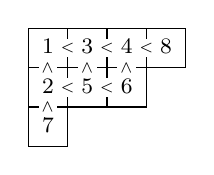
\begin{tikzpicture}
            \footnotesize
            \draw
                (0,0) -- (0,1.5) -- (2,1.5) -- (2,1) -- (1.5,1) -- (1.5,0.5) -- (0.5,0.5) -- (0.5,0) -- cycle
                (0,0.5) -- ++(0.5,0)
                (0,1) -- ++(1.5,0)
                (0.5,0.5) -- ++(0,1)
                (1,0.5) -- ++(0,1)
                (1.5,1) -- ++(0,0.5)
            ;
    
            \begin{scope}[text height=1.5ex,text depth=0.25ex]
                \begin{scope}[every node/.style={fill=white,inner sep=1.5pt}]
                    \tiny
                    \node at (0.5,1.25) {$<$};
                    \node at (1  ,1.25) {$<$};
                    \node at (1.5,1.25) {$<$};
                    \node at (0.5,0.75) {$<$};
                    \node at (1  ,0.75) {$<$};
        
                    \node [rotate=-90] at (0.25,1)   {$<$};
                    \node [rotate=-90] at (0.75,1)   {$<$};
                    \node [rotate=-90] at (1.25,1)   {$<$};
                    \node [rotate=-90] at (0.25,0.5) {$<$};
                \end{scope}
    
                \node at (0.25,0.25) {7};
                \node at (0.25,0.75) {2};
                \node at (0.25,1.25) {1};
                \node at (0.75,0.75) {5};
                \node at (0.75,1.25) {3};
                \node at (1.25,0.75) {6};
                \node at (1.25,1.25) {4};
                \node at (1.75,1.25) {8};
            \end{scope}
        \end{tikzpicture}
        \caption{Example standard Young tableau.}
        \label{fig:SYTex}
    \end{figure}
    \begin{itemize}
        \item We start with a Young diagram.
        \item We need to fill it with 8 numbers.
        \item There are relations between the boxes.
        \item There are some constraints on what can go where, but multiple fillings are still possible.
        \item In total, there are three $\SYT_8$.
        \item Denote by $T$ a tableau within this set of three.
    \end{itemize}
    \item Theorem: $\dim V_\lambda$ is the number of SYTs of shape $\lambda$.
    \item Examples.
    \begin{figure}[h!]
        \centering
        \begin{subfigure}[b]{0.15\linewidth}
            \centering
            \begin{ytableau}
                1\\
                2\\
                3\\
                4\\
            \end{ytableau}
            \caption{$\Delta(1234)$.}
            \label{fig:SYT4a}
        \end{subfigure}\\[1em]
        \begin{subfigure}[b]{0.15\linewidth}
            \centering
            \begin{ytableau}
                1 & 3 & 4\\
                2\\
            \end{ytableau}
            \caption{$(x_1-x_2)$.}
            \label{fig:SYT4b}
        \end{subfigure}
        \begin{subfigure}[b]{0.15\linewidth}
            \centering
            \begin{ytableau}
                1 & 2 & 4\\
                3\\
            \end{ytableau}
            \caption{$(x_1-x_3)$.}
            \label{fig:SYT4c}
        \end{subfigure}
        \begin{subfigure}[b]{0.15\linewidth}
            \centering
            \begin{ytableau}
                1 & 2 & 3\\
                4\\
            \end{ytableau}
            \caption{$(x_1-x_4)$.}
            \label{fig:SYT4d}
        \end{subfigure}\\[1em]
        \begin{subfigure}[b]{0.23\linewidth}
            \centering
            \begin{ytableau}
                1 & 2\\
                3 & 4\\
            \end{ytableau}
            \caption{$(x_1-x_3)(x_2-x_4)$.}
            \label{fig:SYT4e}
        \end{subfigure}
        \begin{subfigure}[b]{0.23\linewidth}
            \centering
            \begin{ytableau}
                1 & 3\\
                2 & 4\\
            \end{ytableau}
            \caption{$(x_1-x_2)(x_3-x_4)$.}
            \label{fig:SYT4f}
        \end{subfigure}
        \caption{Standard Young tableaux of $m\lambda=4$.}
        \label{fig:SYT4}
    \end{figure}
    \begin{enumerate}
        \item Only ONE way to fill trivial and alternating Young diagrams.
        \item Three ways to fill $(3,1)$.
        \item Two ways to fill $(2,2)$.
    \end{enumerate}
    \item Tip: Learn the representations of $S_4$ by heart!
    \begin{itemize}
        \item Good for the final and in general.
    \end{itemize}
    \item We denote the Specht polynomial written from a standard Young tableau by $\Sp(T)$.
    \begin{itemize}
        \item Given an SYT $T$, $\Sp(T)$ is the product of the Vandermonde determinants for each column where the numbers in the column tell you which variables to plug into said determinant.
        \item For example, the captions of each subfigure in Figure \ref{fig:SYT4} are $\Sp(T)$ for the SYT depicted therein.
    \end{itemize}
    \item We now build up to proving the theorem.
    \item Lemma: Fix a symmetric group $S_n$ and a partition $\lambda\vdash n$. Then the collection $\{\Sp(T)\}$ of Specht polynomials written from all $T\in\SYT_\lambda$ (that is, all standard Young tableaux $T$ of shape $\lambda$) is linearly independent.
    \begin{proof}
        The basic reason that this lemma is true is that each $\Sp(T)$ contains a certain monomial that none of the others contain; specifically, this will be the lexicographically smallest monomial $SM$. To get started, fix $\Sp(T)$, and consider $SM[\Sp(T)]$. Our goal is to reconstruct $T$ from it. In this argument, we will look at a representative example instead of a formal proof. In particular, we will look at the example from Figure \ref{fig:SYTex}. Let's begin.\par
        First off, note that we have an analogous lemma to last time, i.e., we have
        \begin{equation*}
            SM(PQ) = SM(P)SM(Q)
        \end{equation*}
        Reading from Figure \ref{fig:SYTex}, we have
        \begin{equation*}
            \Sp(T) = \Delta(x_1,x_2,x_7)\Delta(x_3,x_5)\Delta(x_4,x_6)
        \end{equation*}
        By considering the determinant interpretation of each Vandermonde determinant, we can determine by inspection that the lexicographically smallest monomial. Essentially, the smallest combinations lie along the diagonal of the matrix:
        \begin{figure}[h!]
            \centering
            \begin{tikzpicture}
                \footnotesize
                \matrix [matrix of math nodes,left delimiter=|,right delimiter=|,every outer matrix/.append style={inner sep=0pt},row 1 column 1/.style={nodes={circle,fill=blz,inner sep=0pt,minimum size=7mm}},row 2 column 2/.style={nodes={circle,fill=blz,inner sep=0pt,minimum size=7mm}},row 3 column 3/.style={nodes={circle,fill=blz,inner sep=0pt,minimum size=7mm}}] {
                    1 & 1 & 1\\
                    x_1 & x_2 & x_7\\
                    x_1^2 & x_2^2 & x_7^2\\
                };
                \node at (1.4,0) {$\cdot$};
                \matrix at (2.4,0) [matrix of math nodes,left delimiter=|,right delimiter=|,every outer matrix/.append style={inner sep=0pt},row 1 column 1/.style={nodes={circle,fill=blz,inner sep=0pt,minimum size=7mm}},row 2 column 2/.style={nodes={circle,fill=blz,inner sep=0pt,minimum size=7mm}}] {
                    1 & 1\\
                    x_3 & x_5\\
                };
                \node at (3.4,0) {$\cdot$};
                \matrix at (4.4,0) [matrix of math nodes,left delimiter=|,right delimiter=|,every outer matrix/.append style={inner sep=0pt},row 1 column 1/.style={nodes={circle,fill=blz,inner sep=0pt,minimum size=7mm}},row 2 column 2/.style={nodes={circle,fill=blz,inner sep=0pt,minimum size=7mm}}] {
                    1 & 1\\
                    x_4 & x_6\\
                };
            \end{tikzpicture}
            \caption{Determining the lexicographically smallest monomial.}
            \label{fig:lexicoSM}
        \end{figure}
        Thus, we have
        \begin{equation*}
            SM[\Sp(T)] = (1\cdot x_2\cdot x_7^2)(1\cdot x_5)(1\cdot x_6)
            = x_2x_7^2x_5x_6
        \end{equation*}
        From this monomial, we can reconstruct the SYT by putting $x_7$ in the bottom by necessity, then we have to put $2,5,6$ (other coefficients of SM) above in the certain order to get the right ordering. Then, we have to put the ones that aren't there ($x_1^0x_3^0x_4^0x_8^0)$ in the top row. This gives us our YT back.
    \end{proof}
    \item Theorem: $\dim V_\lambda=|\SYT_\lambda|$.
    \begin{proof}
        Since the $\Sp(T)$ are linearly independent by the lemma, $\dim V_\lambda\geq|\SYT_\lambda|$. Additionally, the $\Sp(T)$ span $V_{\lambda'}$ because\dots (Rudenko will not finish this proof.)
    \end{proof}
    \item Corollary: $\dim V_\lambda=\dim V_{\lambda'}$.
    \begin{proof}
        Any representation of $S_n$ will be self-dual. Essentially, because partition inversion only induces a transposition of the Young tableau and a transposed SYT is still standard, the number of SYTs will remain fixed under inversion, so so will the quantity its equal to by the above theorem, namely $\dim V_\lambda$.
    \end{proof}
    \item Fact: We have the following identity.
    \begin{equation*}
        V_{\lambda'} = V_\lambda\otimes(\text{sign})
    \end{equation*}
    \item Let $f_\lambda$ be the number of SYTs of shape $\lambda$. We have shown that $f_\lambda\leq\dim(V_\lambda)$.
    \item Theorem (RSK): There exists a bijection between permutations in $S_n$ and pairs of SYTs of the same shape (i.e., of \textbf{area} $n$).
    \begin{itemize}
        \item RSK stands for Robinson-Schensted-Knuth.
        \item Errata??: According to \href{https://en.wikipedia.org/wiki/Robinson%E2%80%93Schensted_correspondence}{Wikipedia}, this theorem (as stated) is the Robinson-Schensted correspondence, a special case of and predecessor to the RSK correspondence that trades under its own name.
    \end{itemize}
    \item Corollary: $f_\lambda=\dim V_\lambda$.
    \begin{proof}
        $\sum_{\lambda=\text{YT of area }n}f_\lambda^2
        = n!
        = \sum(\dim V_\lambda^2)$.
        This proves that $f_\lambda\leq\dim V_\lambda$ and $f_\lambda=\dim V_\lambda$.
    \end{proof}
    \begin{itemize}
        \item What's the difference between this and the previous theorem?? And how does this proof work?
    \end{itemize}
    \item Let's see how the RSK correspondence works through an example.
    \begin{itemize}
        \item Consider the permutation
        \begin{equation*}
            \sigma = (13)(27654) =
            \begin{pmatrix}
                1 & 2 & 3 & 4 & 5 & 6 & 7 & 8\\
                3 & 7 & 1 & 2 & 4 & 5 & 6 & 8\\
            \end{pmatrix}
            \in S_8
        \end{equation*}
        \item We will construct two SYTs of identical shape from $\sigma$.
        \item Start with a pair of empty YTs.
        \begin{center}
            \begin{tikzpicture}
                \path (0,0) -- (5,0);
                \node [right] at (0,0) {\ydiagram{1}};
                \node [right] at (3,0) {\ydiagram{1}};
            \end{tikzpicture}
        \end{center}
        \begin{itemize}
            \item We will call the left one the \textbf{insertion tableau} and the right one the \textbf{recording tableau}.
        \end{itemize}
        \item Fill $\sigma(1)=3$ into the insertion tableau and record that this is the first (1) number inserted in the corresponding box of the recording tableau.
        \begin{center}
            \begin{tikzpicture}
                \path (0,0) -- (5,0);
                \node [right] at (0,0) {\ytableaushort{3}};
                \node [right] at (3,0) {\ytableaushort{1}};
            \end{tikzpicture}
        \end{center}
        \item We now have a new pair of tableaux. How do we insert the next number $\sigma(2)=7$? Try adding it to the right of 3 in the insertion tableau. Record this addition in the recording tableau by adding to it a new box in the same relative position as the new 7 box and filling it with 2.
        \begin{center}
            \begin{tikzpicture}
                \path (0,0) -- (5,0);
                \node [right] at (0,0) {\ytableaushort{37}};
                \node [right] at (3,0) {\ytableaushort{13}};
            \end{tikzpicture}
        \end{center}
        \item How do we insert the next number $\sigma(3)=1$? In the insertion tableau, push out 3 with 1 and move 3 to the next row. In the recording tableau, add a new square in the corresponding bottom position and fill it with 3.
        \begin{center}
            \begin{tikzpicture}
                \path (0,0) -- (5,0);
                \node [right] at (0,0) {\ytableaushort{17,3}};
                \node [right] at (3,0) {\ytableaushort{12,3}};
            \end{tikzpicture}
        \end{center}
        \item Next number: 2 pushes out 7 in the insertion tableau. 4 goes in the new box in the recording tableau.
        \begin{center}
            \begin{tikzpicture}
                \path (0,0) -- (5,0);
                \node [right] at (0,0) {\ytableaushort{12,37}};
                \node [right] at (3,0) {\ytableaushort{12,34}};
            \end{tikzpicture}
        \end{center}
        \item 4 gets inserted to the right; 5 fills the new box.
        \begin{center}
            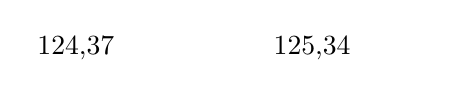
\begin{tikzpicture}
                \path (0,0) -- (5,0);
                \node [right] at (0,0) {\ytableaushort{124,37}};
                \node [right] at (3,0) {\ytableaushort{125,34}};
            \end{tikzpicture}
        \end{center}
        \item 5,6,8 go further to the right; 6,7,8 in the second one.
        \begin{center}
            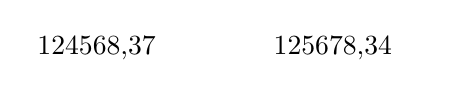
\begin{tikzpicture}
                \path (0,0) -- (5,0);
                \node [right] at (0,0) {\ytableaushort{124568,37}};
                \node [right] at (3,0) {\ytableaushort{125678,34}};
            \end{tikzpicture}
        \end{center}
        \item Now we have a pair of standard Young tableaux.
    \end{itemize}
    \item For every permutation, the above algorithm gives us a pair of SYTs.
    \item Formally, we are following the \href{https://en.wikipedia.org/wiki/Robinson%E2%80%93Schensted_correspondence}{Schensted row-insertion algorithm}, formalized as follows.
    \begin{figure}[H]
        \centering
        \includegraphics[width=0.2\linewidth]{SchenstedAlgorithm.png}
        \caption{The Schensted algorithm.}
        \label{fig:SchenstedAlgorithm}
    \end{figure}
    \begin{enumerate}
        \item Begin with an insertion tableau and a new number to insert. The new number must not appear anywhere in the insertion tableau.
        \item Find the smallest number in row one that is greater than the new number. If no such number exists, append the new number to the end of the row, and we are done. If such a number does exist, replace it with the new number and prepare to insert the number that just got replaced into row two.
        \item In the same manner as Step 2, find the smallest number in row two that is greater than the number that just got replaced. Replace it and move onto the third row.
        \item Keep repeating until we reach a row where we can append the number from the previous row to the end of the line. If no such row exists, eventually we will reach the bottom of the Young tableau and we may start a new row.
    \end{enumerate}
    % \item Why does this work?
    % \begin{itemize}
    %     \item Everything is increasing in rows.
    %     \item If $y>x$, we need to insert it in the row below but to the left.
    %     \item Perhaps its starting with $y$ in the top row and then it being displaced down and to the left by $x$.
    %     \item Every time we add something bigger, we add a corner box.
    %     \item This algorithnm proves the theorem.
    %     \item I really need to think about this!!
    % \end{itemize}
    \item This algorithm provides a constructive proof of the RSK theorem.
    \begin{itemize}
        \item In particular, this algorithm takes us between a pair $(T,T')$ of Young tableaux and a permutation $\sigma$.
    \end{itemize}
    \item This map has many interesting properties that are hard to prove. Here's a few.
    \begin{enumerate}
        \item The map takes $(T',T)\mapsto\sigma^{-1}$.
        \item $\lambda_1$ and $\lambda_1'$ are the length of the longest increasing (resp. decreasing) subsequence of your permutation variables.
    \end{enumerate}
    \item Last word: There is a famous theorem called the \textbf{Erd\H{o}s-Szekeres theorem}.
    \begin{itemize}
        \item This correspondence is a deep way to understand permutations/sequences of numbers. This is a big tool in CS.
    \end{itemize}
    \item Next time: Induction and restriction.
\end{itemize}



\section{Induction and Restriction}
\begin{itemize}
    \item \marginnote{11/17:}Review: Representations of $S_n$.
    \begin{itemize}
        \item $\lambda$ is a partition.
        \item $V_\lambda$ is the span of $\Sp_\lambda(x_1,\dots,x_n)$.
        \item $\dim V_\lambda=\#\SYT_\lambda$, i.e., equals the number of standard Young tableaux of shape $\lambda$.
    \end{itemize}
    \item Naturally, it is desirable to find a better way of counting $\SYT_\lambda$. We will do this with the \textbf{hook length formula}.
    \item \textbf{Hook length formula}: The formula given as follows, where $n$ is the number being partitioned. \emph{Given by}
    \begin{equation*}
        \#\SYT_\lambda = \frac{n!}{\prod\text{length of all hooks}}
    \end{equation*}
    \begin{itemize}
        \item We should feel free to use this formula, but know that it's quite difficult to prove, so Rudenko will forego such a proof.
    \end{itemize}
    \item \textbf{Hook} (of a cell): The set of all cells in a Young diagram directly to the right of or directly beneath the cell in question, including the cell in question.
    \item \textbf{Length} (of a hook): The cardinality of the hook in question.
    \item Example.
    \begin{figure}[h!]
        \centering
        \begin{ytableau}
            7 & 4 & 3 & 1\\
            5 & 2 & 1\\
            2\\
            1\\
        \end{ytableau}
        \caption{Hook length formula.}
        \label{fig:hookLengthForm}
    \end{figure}
    \begin{itemize}
        \item The Young diagram in Figure \ref{fig:hookLengthForm} corresponds to the partition $9=(4,3,1,1)$.
        \item In each cell of the diagram is the length of the hook corresponding to that cell.
        \item Thus, using the hook length formula, the number of standard Young tableaux of shape $(4,3,1,1)$ is
        \begin{equation*}
            \frac{9!}{7\cdot 4\cdot 3\cdot 1\cdot 5\cdot 2\cdot 1\cdot 2\cdot 1} = 9\cdot 8\cdot 3
            = 216
        \end{equation*}
    \end{itemize}
    \item We're headed toward \textbf{branching}.
    \item We'll cover \textbf{induction} and \textbf{restriction} first.
    \begin{figure}[h!]
        \centering
        \begin{tikzpicture}
            \footnotesize
            \draw [blx] (0,1) ellipse (1cm and 0.6cm);
            \foreach \x in {1,...,6} {
                \fill [bly,yshift=1cm] ({0.7*rand},{0.4*rand}) circle (2pt);
            }
            \draw [blx] (0,-1) ellipse (1cm and 0.6cm);
            \foreach \x in {1,...,6} {
                \fill [bly,yshift=-1cm] ({0.7*rand},{0.4*rand}) circle (2pt);
            }
    
            \draw [->] (0.5,-0.3) -- node[right]{$\ind_H^G$} (0.5,0.3);
            \draw [<-] (-0.5,-0.3) -- node[left]{$\res_H^G$} (-0.5,0.3);
        \end{tikzpicture}
        \caption{Induction and restriction as functors.}
        \label{fig:induceFunctor}
    \end{figure}
    \begin{itemize}
        \item These are pretty natural things related to group $G$ and subgroup $H\leq G$.
        \item Essentially, we have $G$-reps and $H$-reps, and we want to interconvert between them.
        \item Induction allows you to go from $H$-reps up to $G$-reps, and vice versa for restrictions.
        \item In category theory, we call these maps \textbf{functors}.
        \begin{itemize}
            \item Now would be a good time to dive into the definition of functor a bit more deeply!
        \end{itemize}
    \end{itemize}
    \item The map down is denoted by $\res_H^G$, and the map up is denoted by $\ind_H^G$.
    \item \textbf{Restriction} (of $V$ to $H\leq G$): The vector space $V$ viewed as an $H$-representation, i.e., a straight-up functional restriction of $\rho_V$. \emph{Denoted by} $\bm{\res_H^G(V)}$.
    \item Example: Consider $S_2<S_3$. Find $\res_{S_2}^{S_3}(2,1)$.
    \begin{itemize}
        \item Recall that $(2,1)=\inp{x_1-x_2,x_1-x_3}$, so this is our answer.
        \item However, suppose we want to express $(2,1)$ in a form that tells us a bit more about its status as an $S_2$-representation. In particular, while $(2,1)$ was an irrep of $S_3$, it is \emph{not} an irrep of $S_2$. Indeed, the group $S_2$ is abelian and hence only has one-dimensional irreps, so we should be able to decompose $(2,1)$ into a sum of two invariant subspaces.
        \item So, looking at polynomials fixed and flipped under $S_2$, we obtain
        \begin{equation*}
            \res_{S_2}^{S_3}(2,1) = \inp{x_1-x_2}\oplus\inp{x_1-x_3+x_2-x_3}
        \end{equation*}
        \begin{itemize}
            \item The left polynomial flips under $S_2$. Specifically, $(12)\cdot(x_1-x_2)=(x_2-x_1)=-(x_1-x_2)$.
            \item The right polynomial stays the same under $S_2$. Specifically, $(12)\cdot(x_1-x_3+x_2-x_3)=(x_2-x_3+x_1-x_3)=(x_1-x_3+x_2-x_3)$.
            \item Obviously, neither polynomial changes under $e$.
            \item Note also that adding the right and left polynomials yields $2(x_1-x_3)\in\spn(2,1)$, as expected.
        \end{itemize}
        \item Let's highlight a few other features of this decomposition.
        \item The two representations in the decomposition are the alternating and trivial --- $(1,1)$ and $(2)$ --- respectively.
        \item While it is fairly obvious that $x_1-x_2$ --- one of the basis vectors of $(2,1)$ --- is the basis for the alternating subrepresentation, finding the other one by inspection is trickier. Thus, here's a procedural way to do it.
        \begin{itemize}
            \item Since the subspaces fixed under $(12)$ are just its eigenspaces, let's compute the eigenvectors of the transformation.
            \item Let $a:=x_1-x_2$ and $b:=x_1-x_3$.
            \item Observe that
            \begin{align*}
                (12)\cdot a &= x_2-x_1 = -(x_1-x_2) = -a\\
                (12)\cdot b &= x_2-x_3 = (x_1-x_3)-(x_1-x_2) = b-a
            \end{align*}
            \item Thus,
            \begin{equation*}
                \rho_{(2,1)}(12) =
                \begin{bmatrix}
                    -1 & -1\\
                    0 & 1\\
                \end{bmatrix}
            \end{equation*}
            \begin{itemize}
                \item Letting $(1,0)=a$ and $(0,1)=b$, we have
                \begin{align*}
                    \underbrace{
                        \begin{bmatrix}
                            -1 & -1\\
                            0 & 1\\
                        \end{bmatrix}
                    }_{\rho_{(2,1)}(12)}\underbrace{
                        \begin{bmatrix}
                            1\\
                            0\\
                        \end{bmatrix}
                    }_a &= \underbrace{
                        \begin{bmatrix}
                            -1\\
                            0\\
                        \end{bmatrix}
                    }_{-a}&
                    \underbrace{
                        \begin{bmatrix}
                            -1 & -1\\
                            0 & 1\\
                        \end{bmatrix}
                    }_{\rho_{(2,1)}(12)}\underbrace{
                        \begin{bmatrix}
                            0\\
                            1\\
                        \end{bmatrix}
                    }_a &= \underbrace{
                        \begin{bmatrix}
                            -1\\
                            1\\
                        \end{bmatrix}
                    }_{b-a}
                \end{align*}
                as expected.
            \end{itemize}
            \item Computing the eigenvectors of this matrix, we obtain
            \begin{align*}
                e_1 &= \underbrace{
                    \begin{bmatrix}
                        1\\
                        0\\
                    \end{bmatrix}
                }_a&
                e_2 &= \underbrace{
                    \begin{bmatrix}
                        -1\\
                        2\\
                    \end{bmatrix}
                }_{2b-a}
            \end{align*}
            \item Plugging in the original definitions of $a,b$, we obtain
            \begin{align*}
                e_1 &= x_1-x_2\\
                e_2 &= 2(x_1-x_3)-(x_1-x_2) = x_1-x_3+x_2-x_3
            \end{align*}
            as expected.
        \end{itemize}
        \item If we treat $x_1,x_2,x_3$ as the standard basis of $\R^3$, then $x_1-x_2$ and $x_1-x_3$ do span a plane containing $x_1-x_3+x_2-x_3$, as we can prove with vector algebra. Moreover, as we would expect for a direct sum, $x_1-x_2$ and $x_1-x_3+x_2-x_3$ are orthogonal:
        \begin{equation*}
            \underbrace{
                \begin{bmatrix}
                    1\\
                    -1\\
                    0\\
                \end{bmatrix}
            }_{x_1-x_2}\cdot\underbrace{
                \begin{bmatrix}
                    1\\
                    1\\
                    -2\\
                \end{bmatrix}
            }_{x_1-x_3+x_2-x_3}
            = (1)(1)+(-1)(1)+(0)(-2)
            = 0
        \end{equation*}
        \item Moreover, the action of $(12)$ on 3D space (i.e., with standard basis $x_1,x_2,x_3$) is a reflection along $x_1-x_2$ and through the plane containing $x_1-x_3+x_2-x_3$; this really shows how $(12)$ fixes both axes while "flipping" one.
    \end{itemize}
    \item We now move onto induction.
    \item Induction is highly nontrivial. It is one of those things in math that is just very tricky. All definitions of it are slightly uncomfortable.
    \item Here's a first attempt at a definition.
    \begin{itemize}
        \item Let $H\acts W$ as an $H$-rep.
        \item We want to create a $G$-rep $\ind_H^GW$.
        \item To start, let's decompose $G$ into left cosets via
        \begin{equation*}
            G = g_1H\sqcup g_2H\sqcup\cdots\sqcup g_kH
        \end{equation*}
        \begin{itemize}
            \item Suppose $g_1\in H$ so that $g_1H=H$.
        \end{itemize}
        \item $\ind_H^GW$ is defined as the vector space $g_1W\oplus\cdots\oplus g_kW$. As a vector space, each $g_iW=W$, but there is additional structure as representations.
        \item Indeed, we must answer the question, "how does $g$ act on $g_iw$?"
        \item Answer: Via
        \begin{equation*}
            g\cdot(g_iw) = g_{\sigma(i)}h_iw
            = g_{\sigma(i)}(h_iw)
        \end{equation*}
        \begin{itemize}
            \item The first equality comes from defining $\sigma\in S_n$ and $h_i\in H$ so that $gg_i=g_{\sigma(i)}h_i$.
            \item We have this equality because $gg_i\in G$, so $gg_i\in\bigsqcup g_iH$, so for some $j=\sigma(i)$, $gg_i\in g_jH=g_{\sigma(i)}H$, i.e., $gg_i=g_{\sigma(i)}h_i$ for some $h_i\in H$.
            \item Note that in the last part of the equality, $h_iw$ is the action of $h_i$ on $w$ via the $H$-rep.
        \end{itemize}
        \item So basically, $g$ takes $g_iw$, isolates $w$, acts on it via $h$ using the original representation to make $h_iw$, and then places this element within the subspace $g_{\sigma(i)}W$.
        \item Each element of $G$ acts in a big block-triangular matrix. Inside each block, you will see how $g$ acts on $H$.
    \end{itemize}
    \item Let $W$ be the trivial representation of $H$. Then $\ind_H^G(\id)$ is the permutational representation of $G$ acting on left cosets.
    \begin{itemize}
        \item Example: $\ind_{\{e\}}^G(\id)=\C[G]$.
        \item See Example 2 from Section 3.3 of \textcite{bib:Serre}.
    \end{itemize}
    \item There is a correspondence between $H/\Stab(x)$ and $G$??
    \begin{itemize}
        \item This is the master construction of representations when you have a subgroup.
    \end{itemize}
    \item The dimension of an induced representation can be calculated via
    \begin{equation*}
        \dim\ind_H^GW = (\dim W)(G:H)
    \end{equation*}
    \item A slightly fancier way to think about this stuff, if you're unsatisfied at this point.
    \begin{itemize}
        \item Take $H<G$, and $H$-rep $W$.
        \item Let's look at functions on $G$ with values in $W$, i.e., functions $f:G\to W$. This would be $\Hom_\C(\C[G],W)$, once we've linearized $G$ so that we can consider linear maps. These linear maps are the exact same thing as the original functions because the basis of $\C[G]$ is $G$!
        \item Since we know how to calculate the dimension of a space of homomorphisms, we have $\dim\Hom_\C(\C[G],W)=(|G|)(\dim W)$.
        \item Under this construction, we get to say that
        \begin{equation*}
            \ind_H^GW = \Hom_H(\C[G],W)=\{f:G\to W\mid f(x\cdot h)=f(xh^{-1})=hf(x)\}
        \end{equation*}
        \item We can easily see that this space has the right dimension; such a function is uniquely defined by its values on $g_1,\dots,g_k$.
        \begin{itemize}
            \item $f(g_1),\dots,f(g_k)$ and $f(g_1h)=h^{-1}f(g_1)$.
        \end{itemize}
        \item What is $g$ acting on in this function? So $[g(f)](x)=f(gx)$...
        \item In this case, it's very easy to see that this is a construction with no choices of $g_i$'s, of cosets, etc. Thus fancier.
    \end{itemize}
    \item Once again, there is no easy way to understand this; we just have to work with it.
    \item Even fancier construction!
    \begin{itemize}
        \item Let $W$ be an $H$-representation. Abstractly, this means that $W$ is a module over $\C[H]$.
        \item Take $W\otimes_{\C[H]}\C[G]$.
        \begin{itemize}
            \item Essentially, this means that if $w\otimes g$, then $hw\otimes g=w\otimes g$.
        \end{itemize}
        \item This has something to do with the second representation.
        \item This is the most abstractly nice construction because it's much more general.
        \begin{itemize}
            \item We don't need to use it on groups; we can use it on algebras and modules over them.
            \item Indeed, this works in complete generality and has all the same properties.
            \item Takeaway: This induced representation is something very, very general, but thinking of it more generally does not help you understand it to start.
        \end{itemize}
    \end{itemize}
    \item We will do a bunch of computations of such \textbf{induced representations} on the homework.
    \item Theorem (Frobenius): Let $H<G$, and let $W$ be an $H$-rep. Then
    \begin{equation*}
        \chi_{\ind_H^GW}(g) = \frac{1}{|H|}\sum_{\substack{x\in G\\g_i^{-1}gg_i\in H}}\chi_W(g_i^{-1}gg_i)
    \end{equation*}
    \item Discussion.
    \begin{itemize}
        \item Look at the picture from the blackboard.
        \begin{itemize}
            \item Characters are class functions; they don't change under conjugation.
        \end{itemize}
        \item $\chi_W$ is a class function in $H$. An alternate formulation of the formula can be obtained by extending the $\chi_W$ (which is a class function in $H$) to $\tilde{\chi}_W$ (which is a class function in $G$).
        \begin{itemize}
            \item We could extend it to $\chi_W:G\to\C$ via
            \begin{equation*}
                \tilde{\chi}_W =
                \begin{cases}
                    0 & g\notin H\\
                    \chi_W(g) & g\in H
                \end{cases}
            \end{equation*}
            \item From here, take
            \begin{equation*}
                \chi_{\ind_H^GW} = \frac{1}{|H|}\sum_{x\in G}\tilde{\chi}_W(xgx^{-1})
            \end{equation*}
            \item So we're basically just averaging again.
        \end{itemize}
    \end{itemize}
    \item Proof: See Theorem \ref{trm:induceChi} from Section 3.3 of \textcite{bib:Serre}.
    % \begin{proof}
    %     We basically just need to understand the cosets construction from above.
        
    %     Let $G=g_1H\oplus\cdots\oplus g_kH$. There is a bigger block matrix that has $(\dim W)\times(\dim W)$ blocks. Then
    %     \begin{equation*}
    %         \chi_{\ind}(g) = \sum_{\substack{gg_i=g_ih\\g_i^{-1}gg_i\in H}}\chi_W(g_i^{-1}gg_i)
    %     \end{equation*}
    %     This gets us back to the above somehow.
    % \end{proof}
    \item Next week:
    \begin{itemize}
        \item If we want to construct $\res_{S_{n-1}}^{S_n}$, we will take all diagrams inside the Young diagram but one box less.
        \item For example,
        \begin{equation*}
            \res_{S_{n-1}}^{S_n}\tikz[baseline={(0,-0.1)}]{\node{\ydiagram{3,2,1,1}};}
            = \tikz[baseline={(0,-0.25)}]{\node{\ydiagram{3,2,1}};}
            \oplus\tikz[baseline={(0,-0.1)}]{\node{\ydiagram{3,1,1,1}};}
            \oplus\tikz[baseline={(0,-0.1)}]{\node{\ydiagram{2,2,1,1}};}
        \end{equation*}
        \item This is the branching rules.
        \item New HW will appear soon and be due Friday of Week 9.
        \begin{itemize}
            \item Will be a bit harder (some hands-on, some fancy); if you can't do everything there, don't worry.
        \end{itemize}
        \item Midterms will be returned early after Thanksgiving.
        \item Final will include some stuff from the last HW, but it will be easier.
    \end{itemize}
\end{itemize}



\section{S Chapter 3: Subgroups, Products, Induced Representations}
\emph{From \textcite{bib:Serre}.}
\setcounter{theorem}{8}
\subsection*{Section 3.1: Abelian Subgroups}
\begin{itemize}
    \item \marginnote{12/28:}Definition of \textbf{abelian}/\textbf{commutative} (group).
    \item Irreducible representations of abelian groups.
    \begin{theorem}\label{trm:irrepAbelianG}
        The following properties are equivalent:
        \begin{enumerate}[label={\textup{(\roman*)}}]
            \item $G$ is abelian.
            \item All the irreducible representations of $G$ have degree 1.
        \end{enumerate}
        \begin{proof}
            Let $n_1,\dots,n_h$ be the degrees of the distinct irreducible representations of $G$. Recall that
            \begin{equation*}
                |G| = \sum_{i=1}^hn_i^2
            \end{equation*}
            If $G$ is abelian, then there are $|G|$ conjugacy classes and hence $|G|$ irreducible representations. But observe from the above equation that $|G|=h$ iff each $n_i=1$, which implies the theorem.
        \end{proof}
    \end{theorem}
    \begin{itemize}
        \item See Section 1.3 of \textcite{bib:FultonHarris} for an alternate approach to this theorem.
    \end{itemize}
    \item Irreducible representations of abelian subgroups.
    \begin{corollary}
        Let $A$ be an abelian subgroup of $G$. Then each irreducible representation $V$ of $G$ has degree
        \begin{equation*}
            \dim(V) \leq (G:A)
        \end{equation*}
        \begin{proof}
            Let $\rho:G\to GL(V)$ be an irreducible representation of $G$. Through \textbf{restriction} to the subgroup $A$, it defines a representation $\rho_A:A\to GL(V)$ of $A$. Let $W\subset V$ be an irreducible subrepresentation of $\rho_A$; by Theorem \ref{trm:irrepAbelianG}, we have $\dim(W)=1$. Let
            \begin{equation*}
                V' = \bigcup_{g\in G}\rho(g)W
            \end{equation*}
            Since $V'$ is a subspace of $V$ that is clearly stable under $G$ by definition, the fact that $V$ is irreducible implies that $V'=V$. Additionally, we have for any $g\in G$ and $a\in A$ that
            \begin{equation*}
                \rho(ga)W = \rho(g)\rho(a)W = \rho(g)W
            \end{equation*}
            This means that many of the $\rho(g)W$ composing $V'$ are identical; in fact, it is only each \emph{coset} of $G$ with respect to $A$ that can possibly contribute a new dimension to $V'$. Moreover, since $\dim(W)=1$, it will only be at most 1 dimension that any $\rho(g)W$ contributes to the union. Essentially, each of the $(G:A)$ cosets contributes at most one dimension to $V'=V$, so $\dim(V)$ cannot exceed $(G:A)$, as desired.
        \end{proof}
    \end{corollary}
    \item Example: A dihedral group contains a cyclic subgroup of index 2; its irreps thus have degree 1 or 2.
\end{itemize}


\subsection*{Section 3.2: Product of Two Groups}
\begin{itemize}
    \item \textbf{Product} (of $G_1,G_2$): The set of pairs $(s_1,s_2)$ with $s_1\in G_1$ and $s_2\in G_2$. \emph{Denoted by} $\bm{G_1\times G_2}$.
    \item \textbf{Group product} (of $G_1,G_2$): The group $(G_1\times G_2,\cdot)$, where $\cdot$ is the group structure defined by
    \begin{equation*}
        (s_1,s_2)\cdot(t_1,t_2) = (s_1t_1,s_2t_2)
    \end{equation*}
    \emph{Denoted by} $\bm{G_1\times G_2}$.
    \item Properties of $G_1\times G_2$.
    \begin{enumerate}
        \item $|G_1\times G_2|=|G_1|\times|G_2|$.
        \item $G_1\cong\{(s_1,1)\mid s_1\in G_1\}\leq G_1\times G_2$ and $G_2\cong\{(1,s_2)\mid s_2\in G_2\}\leq G_1\times G_2$.
        \item With the identifications in Property 2, each element of $G_1$ commutes with each element of $G_2$.
    \end{enumerate}
    \item These properties characterize $G_1\times G_2$ completely, as we will see immediately below.
    \item \textbf{Direct product} (of $G_1,G_2$): The group $G$ containing $G_1,G_2$ as subgroups and satisfying the conditions\dots
    \begin{enumerate}[label={\textup{(\roman*)}}]
        \item Each $s\in G$ can be written uniquely in the form $s=s_1s_2$ with $s_1\in G_1$ and $s_2\in G_2$;
        \item For $s_1\in G_1$ and $s_2\in G_2$, we have $s_1s_2=s_2s_1$.
    \end{enumerate}
    \emph{Also known as} \textbf{product}.
    \item Equivalence of the direct product with the group product.
    \begin{itemize}
        \item Because of the two conditions, the product of any two $s,t\in G$ can be written as follows.
        \begin{align*}
            st &= (s_1s_2)(t_1t_2)\tag*{Condition (i)}\\
            &= s_1(s_2t_1)t_2\\
            &= s_1(t_1s_2)t_2\tag*{Condition (ii)}\\
            &= (s_1t_1)(s_2t_2)
        \end{align*}
        \item Thus, the group structure of $G$ mirrors that of $G_1\times G_2$, too.
        \item This gives us everything we need to define an isomorphism $G_1\times G_2\to G$ by
        \begin{equation*}
            (s_1,s_2) \mapsto s_1s_2
        \end{equation*}
    \end{itemize}
    \item \textbf{Tensor product} (of $\rho^1:G_1\to GL(V_1),\rho^2:G_2:GL(V_2)$): The linear representation of $G_1\times G_2$ into $V_1\otimes V_2$ defined as follows. \emph{Denoted by} $\bm{\rho^1\otimes\rho^2}$. \emph{Given by}
    \begin{equation*}
        (\rho^1\otimes\rho^2)(s_1,s_2) = \rho^1(s_1)\otimes\rho^2(s_2)
    \end{equation*}
    \item The characters $\chi$ of $\rho^1\otimes\rho^2$, $\chi_1$ of $\rho^1$, and $\chi_2$ of $\rho^2$ are related as follows.
    \begin{equation*}
        \chi(s_1,s_2) = \chi_1(s_1)\cdot\chi_2(s_2)
    \end{equation*}
    \item \textbf{Diagonal} (subgroup of $G\times G$): The set of pairs $(s,s)$ for all $s\in G$.
    \item Note that the representation $\rho^1\otimes\rho^2$ defined above equals the representation denoted $\rho^1\otimes\rho^2$ in Section 1.5 of \textcite{bib:Serre} when $G_1=G_2$ and when it is restricted to the diagonal subgroup of $G\times G$.
    \item Irreducible representations of group products.
    \begin{theorem}\leavevmode
        \begin{enumerate}[label={\textup{(\roman*)}}]
            \item If $\rho^1$ and $\rho^2$ are irreducible, $\rho^1\otimes\rho^2$ is an irreducible representation of $G_1\times G_2$.
            \begin{proof}
                Since $\rho^1,\rho^2$ are irreducible, Theorem \ref{trm:irrepCriterion} implies that
                \begin{align*}
                    \frac{1}{|G_1|}\sum_{s_1\in G_1}|\chi_1(s_1)|^2 &= 1&
                    \frac{1}{|G_2|}\sum_{s_2\in G_2}|\chi_2(s_2)|^2 &= 1
                \end{align*}
                By multiplication, this gives
                \begin{equation*}
                    \frac{1}{|G_1\times G_2|}\sum_{(s_1,s_2)\in G_1\times G_2}|\chi(s_1,s_2)|^2 = 1
                \end{equation*}
                It follows by Theorem \ref{trm:irrepCriterion} that $\rho^1\otimes\rho^2$ is irreducible.
            \end{proof}
            \item Each irreducible representation of $G_1\times G_2$ is isomorphic to a representation $\rho^1\otimes\rho^2$, where $\rho^i$ is an irreducible representation of $G_i$ ($i=1,2$).
            \begin{proof}
                A pair of really elegant proofs are given.
            \end{proof}
        \end{enumerate}
    \end{theorem}
    \item Takeaway: "The above theorem completely reduces the study of representations of $G_1\times G_2$ to that of representations of $G_1$ and representations of $G_2$" \parencite[28]{bib:Serre}.
\end{itemize}


\subsection*{Section 3.3: Induced Representations}
\begin{itemize}
    \item Definition of a \textbf{left coset}, $\bm{G/H}$, and \textbf{index} (of $H$ in $G$).
    \item \textbf{Congruent modulo} ($H$ elements $s,s'\in G$): Two elements $s,s'\in G$ that belong to the same left coset. \emph{Denoted by} $\bm{s'\equiv s\pmod{H}$};
    \begin{itemize}
        \item Alternative definition: $s^{-1}s'\in H$. ($s=gh_1$ and $s'=gh_2$ $\Longrightarrow$ $s^{-1}s'=h_1^{-1}g^{-1}gh_2=h_1^{-1}h_2\in H$.)
    \end{itemize}
    \item \textbf{System of representatives} (of $G/H$): A subset $R\subset G$ containing an element from each left coset of $H$. \emph{Denoted by} $\bm{R}$.
    \item Each $s\in G$ can be written uniquely as $s=rt$ for some $r\in R$ and $t\in H$.
    \item We now build up to defining an \textbf{induced} representation. We will construct the definition abstractly first, and then work through a specific, simple example to illustrate the definition. Let's begin.
    \begin{itemize}
        \item Let $\rho:G\to GL(V)$ be a linear representation of $G$.
        \item Let $\rho_H:H\to GL(V)$ denote the restriction $\rho|_H$ of $\rho$ to $H$, and let $W\subset V$ be a subrepresentation of $\rho_H$, i.e., be stable under $\rho_t$ for all $t\in H$.
        \item Let $\theta:H\to GL(W)$ be the linear representation that acts on $W$ as $\rho_H$ acts on $V$.
        \begin{itemize}
            \item Note that this does \emph{not} mean that $\theta(h)=\rho_H(h)=\rho(h)$; rather, since $\dim W<\dim V$ for a nontrivial case of this construction, $\theta(h)$ will yield a matrix/linear transformation of smaller dimension than $\rho_H(h)$.
            \item See the following example for details.
        \end{itemize}
        \item Let $s\in G$ be arbitrary. Observe that the vector space $\rho_sW$ depends only on the left coset $sH$ of $s$; indeed, if we replace $s$ by $st$ where $t\in H$, then we have $\rho_{st}W=\rho_s\rho_tW=\rho_sW$ since $\rho_tW=W$.
        \item Define a subspace $W_\sigma\subset V$ for each left coset $\sigma$ of $H$ by $W_\sigma=\rho_sW$ for some (it does not matter which) $s\in\sigma$.
        \begin{itemize}
            \item Note that the $\rho_s$ permute the $W_\sigma$. Symbolically, if $W_\sigma=\rho_{s_2}W$, then $\rho_{s_1}W_\sigma=\rho_{s_1}\rho_{s_2}W=\rho_{s_1s_2}W=W_{\sigma'}$ for some coset $\sigma'$ of $H$ to which $s_1s_2$ belongs.
        \end{itemize}
        \item Thus, since each $\rho_s=\rho_{rt}$ moves the $W_\sigma$ around internally via $\rho_t$ and between each other via $\rho_r$, the sum $\sum_{\sigma\in G/H}W_\sigma$ is a subrepresentation of $V$.
    \end{itemize}
    \item We now have all the definitions and tools we need to formally define an induced representation.
    \item \textbf{Induced} (representation $\rho:G\to GL(V)$ by $\theta:H\to GL(W)$ for $H\leq G$): The representation $\rho:G\to GL(V)$ defined above, if $V$ is equal to the sum of the $W_\sigma$ ($\sigma\in G/H$) and if this sum is direct (that is, if $V=\bigoplus_{\sigma\in G/H}W_\sigma$).
    \item Example.
    \begin{itemize}
        \item Let $G=\Z/4\Z$, and let $\rho:\Z/4\Z\to GL(\R^2)$ send $0,1,2,3$ to the $\ang{0},\ang{90},\ang{180},\ang{270}$ rotation matrices. Explicitly, we have
        \begin{align*}
            \rho_0 &=
            \begin{bmatrix}
                1 & 0\\
                0 & 1\\
            \end{bmatrix}&
            \rho_1 &=
            \begin{bmatrix}
                0 & -1\\
                1 & 0\\
            \end{bmatrix}&
            \rho_2 &=
            \begin{bmatrix}
                -1 & 0\\
                0 & -1\\
            \end{bmatrix}&
            \rho_3 &=
            \begin{bmatrix}
                0 & 1\\
                -1 & 0\\
            \end{bmatrix}
        \end{align*}
        \item Let $H=\{0,2\}\cong\Z/2\Z$, and let $W=\spn(1,0)\cong\R$.
        \begin{itemize}
            \item Since $\rho_0(1,0)=(1,0)\in\spn(1,0)$ and $\rho_2(1,0)=(-1,0)\in\spn(1,0)$, $W$ is indeed a subrepresentation that is stable under $\rho_H$.
        \end{itemize}
        \item Let $\theta:\{0,2\}\to GL[\spn(1,0)]$ be defined as follows. Since $\rho_0$ maps the basis vector $(1,0)$ of $\spn(1,0)$ to itself, $\theta_0$ should be the identity as well. Since $\rho_2$ maps the basis vector $(1,0)$ of $\spn(1,0)$ to $(-1,0)$, $\theta_2$ should be the opposite of the identity as well. Altogether,
        \begin{align*}
            \theta_0 &=
            \begin{bmatrix}
                1
            \end{bmatrix}&
            \theta_2 &=
            \begin{bmatrix}
                -1
            \end{bmatrix}
        \end{align*}
        \item Denote the two left cosets of $H$ by $\sigma=0+H$ and $\tau=1+H$. Then 
        \begin{align*}
            W_\sigma &= \rho_0\spn(1,0) = \spn(1,0)&
            W_\tau   &= \rho_1\spn(1,0) = \spn(0,1)
        \end{align*}
        \begin{itemize}
            \item We have the rightmost equality above because of $\rho_1$'s matrix definition, which implies that its action on the basis vector $(1,0)$ of $\spn(1,0)$ is $\rho_1(1,0)=(0,1)$.
        \end{itemize}
        \item Thus, altogether, if $\rho$ is to be the representation induced by $\theta$, we must have
        \begin{equation*}
            V = \bigoplus_{\sigma\in G/H}W_\sigma
            = W_0\oplus W_1
            = \spn(1,0)\oplus\spn(0,1)
        \end{equation*}
    \end{itemize}
    \item Let's go a bit deeper with this example, and see how we could recover $\rho$ if all we started with was $G,H,\theta,W$.
    \begin{itemize}
        \item Define $\sigma=0+H$ and $\tau=1+H$.
        \item Then $W_\sigma=\rho_0W$ and $W_\tau=\rho_1W$.
        \item It follows that $V=W_\sigma\oplus W_\tau$.
        \item We can now define $\rho$'s action on the basis $\{W_\sigma,W_\tau\}$ of $V$.
        \begin{align*}
            \rho_0W_\sigma &= \rho_0(\rho_0W) = \rho_0(\rho_0W) = \rho_0(\theta_0W) = \rho_0W  =  W_\sigma\\
            \rho_0W_\tau   &= \rho_0(\rho_1W) = \rho_1(\rho_0W) = \rho_1(\theta_0W) = \rho_1W  =  W_\tau  \\
            \rho_1W_\sigma &= \rho_1(\rho_0W) = \rho_1(\rho_0W) = \rho_1(\theta_0W) = \rho_1W  =  W_\tau  \\
            \rho_1W_\tau   &= \rho_1(\rho_1W) = \rho_0(\rho_2W) = \rho_0(\theta_2W) = -\rho_0W = -W_\sigma\\
            \rho_2W_\sigma &= \rho_2(\rho_0W) = \rho_0(\rho_2W) = \rho_0(\theta_2W) = -\rho_0W = -W_\sigma\\
            \rho_2W_\tau   &= \rho_2(\rho_1W) = \rho_1(\rho_2W) = \rho_1(\theta_2W) = -\rho_1W = -W_\tau  \\
            \rho_3W_\sigma &= \rho_3(\rho_0W) = \rho_1(\rho_2W) = \rho_1(\theta_2W) = -\rho_1W = -W_\tau  \\
            \rho_3W_\tau   &= \rho_3(\rho_1W) = \rho_0(\rho_0W) = \rho_0(\theta_0W) = \rho_0W  =  W_\sigma
        \end{align*}
        \item If we associate $W_\sigma$ with $(1,0)\in\R^2\cong V$ and $W_\tau$ with $(0,1)\in\R^2\cong V$, then the matrices of $\rho_s$ are those given in the original example above.
    \end{itemize}
    \item Note: To get a nontrivial induced representation in this manner, we must have $W<V$. I.e., in the above example, we could not take $\rho_{\{0,2\}}:G\to GL(\R^2)$ and induce \emph{it} up; rather, we needed to deal with $\rho_{\{0,2\}}:G\to GL(\R)$ and induce it.
    \item Let's now look at a couple of reformulations of the definition of an induced representation.
    \begin{enumerate}
        \item Each $x\in V$ can be written uniquely as $\sum_{\sigma\in G/H}x_\sigma$, with $x_\sigma\in W_\sigma$ for each $\sigma$.
        \item If $R$ is a system of representatives of $G/H$, the vector space $V$ is the direct sum of the $\rho_rW$ with $r\in R$.
    \end{enumerate}
    \item A consequence of the second formulation above is that
    \begin{equation*}
        \dim(V) = \sum_{r\in R}\dim(\rho_rW) = (G:H)\cdot\dim(W)
    \end{equation*}
    \item Examples.
    \begin{enumerate}
        \item If $\rho:G\to GL(V)$ is the regular representation of $G$ and $W$ is the subspace with basis $(e_t)_{t\in H}$, then $\theta:H\to GL(W)$ is the regular representation of $W$ and $\rho$ is induced by $\theta$. This is a fairly straightforward case of adding more dimensions to build up the full representation!
        \item The \textbf{permutation representation} of $G$ associated with $G/H$. $e_H$ is invariant under $H$. The representation of $H$ in the subspace $\C e_H$ is the \textbf{unit representation} of $H$, and this representation induces $\rho$.
        \begin{itemize}
            \item This is a more general case of the example presented above, where I chose $G=\Z/4\Z$ and $H=\Z/2\Z$, and restricted $\C e_H$ to $\R e_h$.
        \end{itemize}
        \item If $\rho_1$ is induced by $\theta_1$ and $\rho_2$ is induced by $\theta_2$, then $\rho_1\oplus\rho_2$ is induced by $\theta_1\oplus\theta_2$.
        \item If $(V,\rho)$ is induced by $(W,\theta)$, and if $W_1$ is a stable subspace of $W$, the subspace $V_1=\sum_{r\in R}\rho_rW_1$ of $V$ is stable under $G$, and the representation of $G$ in $V_1$ is induced by the representation of $H$ in $W_1$.
        \item If $\rho$ is induced by $\theta$, if $\rho'$ is a representation of $G$, and if $\rho_H'$ is the restriction of $\rho'$ to $H$, then $\rho\otimes\rho'$ is induced by $\theta\otimes\rho_H'$.
    \end{enumerate}
    \item \textbf{Permutation representation} (of $G$ associated with $G/H$): The representation $\rho:G\to GL(V)$, where $V=(e_\sigma)_{\sigma\in G/H}$ and $\rho_se_\sigma=e_{s\sigma}$.
    \item We now prove the existence and uniqueness of induced representations.
    \begin{itemize}
        \item While the above examples are specific, explicitly verifiable cases of induced representations, we have not yet proven that an induced representation $(V,\rho)$ exists for \emph{every} $(W,\theta)$.
        \item This is our present goal.
    \end{itemize}
    \item Note: This construction here is related to the intermediately fancy construction of induced representations from Friday's class.
    \item To begin, we first state and prove a lemma that will later be useful in proving the uniqueness of the induced representation.
    \begin{lemma}\label{lem:induceUnique}
        Suppose that $(V,\rho)$ is induced by $(W,\theta)$. Let $\rho':G\to GL(V')$ be a linear representation of $G$, and let $f:W\to V'$ be a linear map such that $f(\theta_tw)=\rho_t'f(w)$ for all $t\in H$ and $w\in W$\footnote{Note that this is not quite a morphism of $G$-representations because only $\rho'$ maps from $G$ --- $\theta$ maps from $H$!}. Then there exists a unique linear map $F:V\to V'$ which extends $f$ and satisfies $F\circ\rho_s=\rho_s'\circ F$ for all $s\in G$.
        \begin{proof}
            We first prove the uniqueness of $F$ so that we can use an aspect of this argument to prove its existence. Let's begin.\par
            To prove that $F$ is unique, it will suffice to give a formula derived from the given constraints that wholly characterizes it on $V$. Let $x\in\rho_sW\subset V$ be arbitrary. Then $\rho_s^{-1}x\in W$, hence
            \begin{equation*}
                F(x) = F(\rho_s\rho_s^{-1})
                = \rho_s'F(\rho_s^{-1}x)
                = \rho_s'f(\rho_s^{-1}x)
            \end{equation*}
            as desired.\par
            To prove that $F$ exists, it will suffice to define it by formula and then show that this formula is well-defined. Let $x\in W_\sigma$ be arbitrary. Define $F(x)$ by $F(x)=\rho_s'f(\rho_s^{-1}x)$ for some $s\in\sigma$, mirroring the above. While it may seem that varying the choice of $s$ could vary the definition of $F$, it actually does not: Replace $s$ by $st$ ($t\in H$) to see that
            \begin{equation*}
                \rho_{st}'f(\rho_{st}^{-1}x) = \rho_s'\rho_t'f(\theta_t^{-1}\rho_s^{-1}x)
                = \rho_s'(\theta_t\theta_t^{-1}\rho_s^{-1}x)
                = \rho_s'f(\rho_s^{-1}x)
            \end{equation*}
            We can then check that $F\circ\rho_s=\rho_s'\circ F$ for all $s\in G$. (How?? \textcite{bib:Serre} says it's easy but I'm not seeing it.)
        \end{proof}
    \end{lemma}
    \item Now we state and prove the full existence and uniqueness result.
    \begin{theorem}\label{trm:induceExiUni}
        Let $(W,\theta)$ be a linear representation of $H$. There exists a linear representation $(V,\rho)$ of $G$ which is induced by $(W,\theta)$, and it is unique up to isomorphism.
        \begin{proof}
            We will prove existence and then uniqueness. Let's begin.\par
            \underline{Existence}: In view of Example 3, we may assume that $\theta$ is irreducible. In this case, $\theta$ is isomorphic to a subrepresentation of the regular representation of $H$, which can be induced to the regular representation of $G$ by Example 1. Then applying Example 4, we conclude that $\theta$, itself, can be inducted.\par
            \underline{Uniqueness}: Let $(V,\rho),(V',\rho')$ be two representations induced by $(W,\theta)$. Since $W$ is a subspace of $V'$, we may consider the linear injection $f:W\to V'$. As an injection, $f$ is the identity on $W$, so for any $t\in H$ and $w\in W$, we have $f(\theta_tw)=\theta_tw=\rho_t'w=\rho_t'f(w)$. Thus, applying Lemma \ref{lem:induceUnique}, we see that there exists a linear map $F:V\to V'$ which is the identity on $W$ and satisfies $F\circ\rho_s=\rho_s'\circ F$ for all $s\in G$. Since $F$ is the identity on $W$, $\im(F)$ contains all the $\rho_s'W$ and thus is isomorphic to $V'$. This combined with the fact that $\dim V'=(G:H)\cdot\dim(W)=\dim V$ proves that $F$ is an isomorphism overall, hence completing the proof.
        \end{proof}
    \end{theorem}
    \item We now discuss the character of an induced representation.
    \item Motivation: Since $(W,\theta)$ determines $(V,\rho)$ up to isomorphism, we should be able to compute $\chi_\rho$ from $\chi_\theta$.
    \item Here's how:
    \begin{theorem}\label{trm:induceChi}
        Let $h$ be the order of $H$ and let $R$ be a system of representatives of $G/H$. For each $u\in G$, we have
        \begin{equation*}
            \chi_\rho(u) = \sum_{\substack{r\in R\\r^{-1}ur\in H}}\chi_\theta(r^{-1}ur)
            = \frac{1}{|H|}\sum_{\substack{s\in G\\s^{-1}us\in H}}\chi_\theta(s^{-1}us)
        \end{equation*}
        In particular, $\chi_\rho(u)$ is a linear combination of the values of $\chi_\theta$ on the intersection of $H$ with the conjugacy class of $u$ in $G$.
        \begin{proof}
            We will proceed from the definition of $\chi_\rho(u)$ as
            \begin{equation*}
                \chi_\rho(u) = \tr_V(\rho_u)
            \end{equation*}
            To begin, consider the matrix of $\rho_u$. Since $\rho_u$ permutes the $\rho_rW$ composing $V$, only spaces $\rho_rW$ that $\rho_u$ maps into themselves (i.e., spaces on the block diagonal of the matrix of $\rho_u$) will affect the trace. More precisely, these are spaces for which $ur=rt$ for some $t\in H$. Observe that this condition can be rewritten $r^{-1}ur\in H$. Thus,
            \begin{equation*}
                \chi_\rho(u) = \sum_{\substack{r\in R\\r^{-1}ur\in H}}\tr_{\rho_rW}(\rho_u|_{\rho_rW})
            \end{equation*}
            Recall that the origin of the condition $ur=rt$ is that we needed $\rho_u\rho_r=\rho_r\theta_t$ with $t=r^{-1}ur\in H$. More specifically, since we only care about the action of $\rho_u$ on $\rho_RW$ right now, we have $\rho_u|_{\rho_rW}\rho_r=\rho_r\theta_t$. It follows since $\tr(ab)=\tr(ba)$ and hence $\tr(aba^{-1})=\tr(b)$ that $\tr(\rho_u|_{\rho_rW})=\tr(\rho_r\theta_t\rho_{r^{-1}})=\tr(\theta_t)=\chi_\theta(t)=\chi_\theta(r^{-1}ur)$, which yields
            \begin{equation*}
                \chi_\rho(u) = \sum_{\substack{r\in R\\r^{-1}ur\in H}}\chi_\theta(r^{-1}ur)
            \end{equation*}
            as desired.\par
            The second formula given for $\chi_\rho(u)$ follows from the first by noting that all elements $s\in G$ in the left coset $rH$ ($r\in R_u$) satisfy $\chi_\theta(s^{-1}us)=\chi_\theta(r^{-1}ur)$.
        \end{proof}
    \end{theorem}
    \item Another property of induced representations discussed further in part II: The \textbf{Frobenius reciprocity formula}, which is given by
    \begin{equation*}
        (f_H\mid\chi_\theta)_H = (f\mid\chi_\rho)_G
    \end{equation*}
\end{itemize}



\section{S Chapter 7: Induced Representations; Mackey's Criterion}
\emph{From \textcite{bib:Serre}.}
\setcounter{proposition}{17}
\subsection*{Section 7.1: Induction}
\begin{itemize}
    \item \marginnote{12/29:}We are now treating $V$ as a $\C[G]$-module and $W$ as a $\C[H]$-submodule of $V$.
    \item Definition of \textbf{induced} representation.
    \item We now reformulate the induction property.
    \item Let $W'$ (defined as follows) be the $\C[G]$-module obtained from $W$ by \textbf{scalar extension} from $\C[H]$ to $\C[G]$.
    \begin{equation*}
        W' = \C[G]\otimes_{\C[H]}W
    \end{equation*}
    \begin{itemize}
        \item The injection $W\to V$ extends by linearity to a $\C[G]$-homomorphism $i:W'\to V$.
        \item There is definitely more for me to understand here in the realm of exactly what a scalar extension is!
    \end{itemize}
    \item We now relate $W'$ to $V$.
    \begin{proposition}
        In order that $V$ be induced by $W$, it is necessary and sufficient that the homomorphism
        \begin{equation*}
            i:\C[G]\otimes_{\C[H]}W\to V
        \end{equation*}
        be an isomorphism.
        \begin{proof}
            This follows (somehow??) from the fact that the elements of the elements of a system of left coset representatives for $H$ form a basis of $\C[G]$ considered as a right $\C[H]$-module.
        \end{proof}
    \end{proposition}
    \item Notes.
    \begin{enumerate}
        \item Update on Theorem \ref{trm:induceExiUni}: Because the tensor product is well-defined, his formulation of the representation induced by $W$ obviously \emph{exists} and \emph{is unique}.
        \begin{itemize}
            \item At this point, \textcite{bib:Serre} introduces the $\int_H^G(W)$ notation.
        \end{itemize}
        \item Update on Lemma \ref{lem:induceUnique}: If $V$ is induced by $W$ and if $E$ is a $\C[G]$-module, we have a canonical isomorphism
        \begin{equation*}
            \Hom^H(W,E) \cong \Hom^G(V,E)
        \end{equation*}
        where $\Hom^G(V,E)$ denotes the vector space of $\C[G]$-homomorphisms of $V$ into $E$, and $\Hom^H(W,E)$ is defined similarly.
        \begin{itemize}
            \item This follows from a property of tensor products.
        \end{itemize}
        \item Induction is transitive: If $G$ is a subgroup of a group $K$, then we have
        \begin{equation*}
            \ind_G^K(\ind_H^G(W)) \cong \ind_H^K(W)
        \end{equation*}
        \begin{itemize}
            \item Two ways to see this: Directly or via the associativity of the tensor product.
        \end{itemize}
    \end{enumerate}
    \item A criterion for when a subspace and subgroup can induce a representation.
    \begin{proposition}
        Let $V$ be a $\C[G]$-module which is a direct sum $V=\bigoplus_{i\in I}W_i$ of vector subspaces permuted \textbf{transitively} by $G$. Let $i_0\in I$, $W=W_{i_0}$, and let $H$ be the \textbf{stabilizer} of $W$ in $G$. Then $W$ is stable under the subgroup $H$ and the $\C[G]$-module $V$ is induced by the $\C[H]$-module $W$.
        \begin{proof}
            Obvious, according to \textcite{bib:Serre}.
        \end{proof}
    \end{proposition}
    \item \textbf{Transitive} (permutation by $G$ on a set $X$): A group action for which the orbit of $x$ is $X$ for some (any) $x\in X$.
    \item \textbf{Stabilizer} (of $W$ in $G$): The set of all $s\in G$ such that $sW=W$.
    \item Note on the proposition: In order to apply it to an irrep $V=\bigoplus W_i$ of $G$, it is enough to check that the $W_i$ are permuted among themselves by $G$; the transitivity condition is automatic because each orbit of $G$ in the set of $W_i$'s defines a subrepresentation of $V$.
    \item \textbf{Monomial} (representation): A representation $V$ for which the $W_i$'s are of dimension 1.
\end{itemize}




\end{document}